
\documentclass[calculator,steamtables,refrigeranttables,psychrometricchart,datasheet,solutions]{exam}
%\documentclass[calculator,datasheet]{exam}
%\documentclass[calculator,datasheet,solutions]{exam}


% The full list of class options are
% calculator : Allows approved calculator use.
% datasheet : Adds a note that data sheet are attached to the exam.
% handbook : Allows the use of the engineering handbook.
% resit : Adds the resit markings to the paper.
% sample : Adds conspicuous SAMPLE markings to the paper
% solutions : Uses the contents of \solution commands (and \solmarks) to generate a solution file

\usepackage{pdfpages}
\usepackage{lscape,comment}

\coursecode{EG5597}%
\coursetitle{Advanced Chemical Engineering}%
\examtime{00.00--00.00}%
\examdate{00}{05}{2014}%
\examformat{Candidates must attempt \textit{all} questions.}

\newcommand{\frc}{\displaystyle\frac}
\newcommand{\br}[1]{\!\left( #1 \right)}
\newcommand{\abs}[1]{\left| #1 \right|}
\newcommand{\fracd}[2]{\frac{\mathrm{d} #1}{\mathrm{d} #2}}
\newcommand{\fracp}[2]{\frac{\partial #1}{\partial #2}}
\renewcommand{\d}[1]{\mathrm{d} #1 }
\newcommand{\Ma}{\mathrm{M\!a}}



\begin{document}

%%%
%%% Question 01 
%%%
\begin{question} %\vspace{-2\baselineskip}

%An agitation vessel is used mix a batch of maleic anhydride (liquid) and chlorine (gas) and need to be kept dry (i.e., no water content) and avoid solidification $\left(T_{\text{melting}}=52.8^{\text{o}}C\right)$. Gaseous chlorine (high pressure) is purified mixing  


\begin{enumerate}[(i)]
%
%%% Matrices
\item The linear system below,
\[\left\{\begin{array}{l}
u + v + w = 2 \\
3u + 3v - w = 6 \\
u -v + w = -1
\end{array}\right.\]
can be represented as $\mathcal{A}{\bf x}=b$. 
\begin{enumerate}[(a)]
\item Calculate $\mathcal{A}^{-1}$ using Gauss-Jordan method.~\marks{5}
%
\solution{Matrix $\mathcal{A}I$, 
\[\left(\begin{array}{c c c | c c c}
1 & 1 & 1 & 1 & 0 & 0 \\
3 & 3 & -1& 0 & 1 & 0 \\
1 &-1 & 1 & 0 & 0 & 1\end{array}\right)\]
can be reduced to $I\mathcal{A}^{-1}$\solmarks{2/5}
\[\left(\begin{array}{c c c | c c c}
1 & 0 & 0 & -1/4 & 1/4 & 1/2 \\
0 & 1 & 0 & 1/2  & 0   & -1/2 \\
0 & 0 & 1 & 3/4 & -1/4 & 0\end{array}\right)\]
with the following steps: \solmarks{3/5}
\begin{itemize}
\item {\it Row 2} = {\it Row 2} + {\it Row 1} $\times (-3)$
\item {\it Row 3} = {\it Row 3} + {\it Row 1} $\times (-1)$
\item Swap {\it Row 3} and {\it Row 2}
\item {\it Row 2} = {\it Row 2} $\times (-2)^{-1}$
\item {\it Row 3} = {\it Row 3} $\times (-4)^{-1}$
\item {\it Row 1} = {\it Row 1} + {\it Row 3} $\times (-1)$
\item {\it Row 1} = {\it Row 1} + {\it Row 2} $\times (-1)$
\end{itemize}
}
%%%
\item If the components of 3$\times$3 matrix $\mathcal{A}$ and solution-vector $b$ are replaced by $a_{ij}=1/(i+j-1)$ (Hilbert matrix) and $b_{i}=(-1)^{i-1}$, respectively, 
\begin{enumerate}
\item Solve the resulting linear system using Jacobi method, 
\begin{displaymath}
x_{i}^{(k+1)}=\frc{1}{a_{11}}\left(b_{i}-\sum\limits_{i\ne j}a_{ij}x_{j}^{(k)}\right)
\end{displaymath}
with 3 iterations.~\marks{3}
%
\solution{The 3$\times$3 Hilbert matrix, $\mathcal{A}$, is~\solmarks{1/8}
\[\left(\begin{array}{c c c}
1   & 1/2 & 1/3 \\ 
1/2 & 1/3 & 1/4 \\
1/3 & 1/4 & 1/5 \end{array}\right)\]
and ${\bf b}=\left(1.0\;-1.0\;1.0\right)^{T}$. The vector-solution for this problem is ${\bf X}=\left(0.5\;\;1.5\;\;0.0\right)^{T}$~\solmarks{3/8}. 
}
%%%
\item Also, develop an algorithm that describes the Jacobi method applied to linear systems.~\marks{5}
%
\solution{Algorithm for the Jacobi method:\\
\begin{tabular}{l l}
{\bf Input:}  & $\mathcal{A}=\left[a_{ij}\right]$, {\bf b}, and initial guess ${\bf X}={\bf x^{(0)}}$, Tolerance $\left(\epsilon\right)$ and maximum \\
              &  number of interations $\left(N_{\text{iter}}\right)$.\\
{\bf Step 1:} & Set $k = 1$ \\
{\bf Step 2:} & While $\left(k\leq N_{\text{iter}}\right)$ \\
{\bf Step 3:} & \;\;\; For $i=1,2,...,n$ \\
              & \hspace{2cm}$x_{i}=a_{ii}^{-1}\left[\sum\limits_{j=1,j\ne i}^{n}\left(-a_{ij}x_{j}^{(0)}\right)+b_{i}\right]$\\
{\bf Step 4:} & \;\;\; If $\left\|{\bf x}-x^{(0)}\right\| < \epsilon \rightarrow$ Output: {\bf X} \\
{\bf Step 5:} & \;\;\; Set $k=k+1$ \\
{\bf Step 6:} & \;\;\; For $i=1,2,...,n\rightarrow$ ${\bf x^{(0)}=x_{i}}$ \\
{\bf Step 7:} & Output: {\bf X} \\
              & {\bf Stop} 
\end{tabular}~\solmarks{5/8}
}
\end{enumerate}
%%%
\end{enumerate}
%%%
%%% PDE
\item Partial differential equations (PDE's) can be represented as,
\begin{displaymath}
a u_{xx} + b u_{xy} + c u_{yy} + d u_{x} + e u_{y} + f = 0
\end{displaymath}
where $a$, $b$, ... $f$ are coefficients.
\begin{enumerate}[(a)]
\item Define parabolic, hyperbolic and elliptic PDE's.~\marks{6}
%
\solution{Changing the independent variables $x=\left(\xi,\eta\right)$ and $y=\left(\xi,\eta\right)$, using the chain rule of differentiation~\solmarks{1/6}
\begin{eqnarray}
&& u_{x}  = u_{\xi}\xi_{x} + u_{\eta}\eta_{x} \nonumber \\
&& u_{y}  = u_{\xi}\xi_{y} + u_{\eta}\eta_{y} \nonumber \\
&& u_{xx} = u_{\xi\xi}\xi_{x}^{2} + 2u_{\xi\eta}\eta_{x}\eta_{x} + u_{\eta\eta}\eta_{x}^{2} + u_{\xi}\xi_{xx} +u_{\eta}\eta_{xx} \nonumber \\
&& u_{yy} = u_{\xi\xi}\xi_{y}^{2} + 2u_{\xi\eta}\eta_{y}\eta_{y} + u_{\eta\eta}\eta_{y}^{2} + u_{\xi}\xi_{yy} +u_{\eta}\eta_{yy} \nonumber \\
&& u_{xy} = u_{\xi\xi}\xi_{x}\xi_{y} + u_{\xi\eta}\left(\xi_{x}\eta_{y} + \xi_{y}\eta_{x}\right) + u_{\eta\eta}\eta_{x}\eta_{y} + u_{\xi}\xi_{xy} + u_{\xi}\eta_{xy} \nonumber
\end{eqnarray}
 and substituting in the PDE:~\solmarks{1/6},
\begin{equation}
A u_{\eta\eta} + B u_{\xi\eta} + C u_{\eta\eta} + D u_{\xi} + E u_{\eta} + F = 0\label{eqn:1}
\end{equation}
with
\begin{eqnarray}
&& A = a \xi_{x}^{2} + b\xi_{x}\xi_{y} + c\xi_{y}^{2} \nonumber \\
&& B = 2a\xi_{x}\eta_{x} + b\left(\xi_{x}\eta_{y} + \xi_{y}\eta_{x}\right) + 2c\xi_{y}\eta_{y} \nonumber \\
&& C = a\eta_{x}^{2} + b\eta_{x}\eta_{y} + c\eta_{y}^{2} \nonumber \\
&& D = d\xi_{x} + e\xi_{y} \nonumber \\
&& E = d\xi_{x} + e\eta_{y} \nonumber \\
&& F = f \nonumber
\end{eqnarray}
We can simplify Eqn.~\ref{eqn:1} if $\xi$ and $\eta$ is chosen to vanish $A$ and $C$,~\solmarks{1/6}
\begin{eqnarray}
a\xi_{x}^{2}  + b\xi_{x}\xi_{y}+c\xi_{y}^{2} = 0 \nonumber \\
a\eta_{x}^{2} + b\eta_{x}\eta_{y} + c\eta_{y}^{2} = 0 \nonumber
\end{eqnarray}
Now,
\begin{itemize}
\item $b^{2}-4ac > 0$: Hyperbolic equation;~\solmarks{1/6}
\item $b^{2}-4ac = 0$: Parabolic equation;~\solmarks{1/6}
\item $b^{2}-4ac < 0$: Elliptic equation.~\solmarks{1/6}
\end{itemize}
}
%%%
\item A particular case of these PDE's is
\begin{displaymath}
u_{t}+\alpha u_{x} = \kappa u_{xx}
\end{displaymath}
that represents advection-diffusion problems (with constant coefficients $\alpha$ and $\kappa$) with a number of applications in fluid and solid mechanics. Demonstrate that the advection term (in 1D and assuming regular grid) is
\begin{displaymath}
\frc{\partial u}{\partial x}=\frc{u_{i+1}-u_{i}}{\Delta x_{i}} + \mathcal{O}\left(\Delta x\right)
\end{displaymath}
using Taylor's expansion.~\marks{6}
%
\solution{Expanding the function $u$ at $x_{i+1}$ about the point $x_{i}$ (assuming regular grid):~\solmarks{2/6}
\begin{displaymath}
u\left(x_{i}+\Delta x_{i}\right) = u\left(x_{i}\right) + \Delta x_{i}\left.\frac{\partial u}{\partial x}\right|_{x_{i}} + \frac{\Delta x_{i}^{2}}{2!}\left.\frac{\partial^{2} u}{\partial x^{2}}\right|_{x_{i}} + \frac{\Delta x_{i}^{3}}{3!}\left.\frac{\partial^{3} u}{\partial x^{3}}\right|_{x_{i}} + \cdot\cdot\cdot
\end{displaymath}
The Taylor expansion can be rearranged as,
\begin{displaymath}
\frac{u\left(x_{i} + \Delta x_{i}\right) - u\left(x_{i}\right)}{\Delta x_{i}} - \left.\frac{\partial u}{\partial x}\right|_{x_{i}} = \frac{\Delta x_{i}^{2}}{2!}\left.\frac{\partial^{2} u}{\partial x^{2}}\right|_{x_{i}} + \frac{\Delta x_{i}^{3}}{3!}\left.\frac{\partial^{3} u}{\partial x^{3}}\right|_{x_{i}} + \cdot\cdot\cdot
\end{displaymath}
The r.h.s of the above equation is the {\bf truncation error} of the series~\solmarks{1/6}, and the equation can be rewritten as,
\begin{displaymath}
\left.\frac{\partial u}{\partial x}\right|_{x_{i}} = \frac{u_{i+1}-u_{i}}{\Delta x_{i}} + \mathcal{O}\left(\Delta x\right)
\end{displaymath}~\solmarks{3/6}


}
%%%
\end{enumerate}

%%% Numerical integration or ODE?
%\item 
%
\end{enumerate}

\end{question}


\clearpage

\paperend

%\begin{comment}
%\begin{landscape}
%\begin{center}
%\includegraphics[width=1.5\textwidth]{PsychrometricChart}
%\end{center}
%{
%  \includepdf[pages=-,fitpaper]{PsychrometricChart}
%  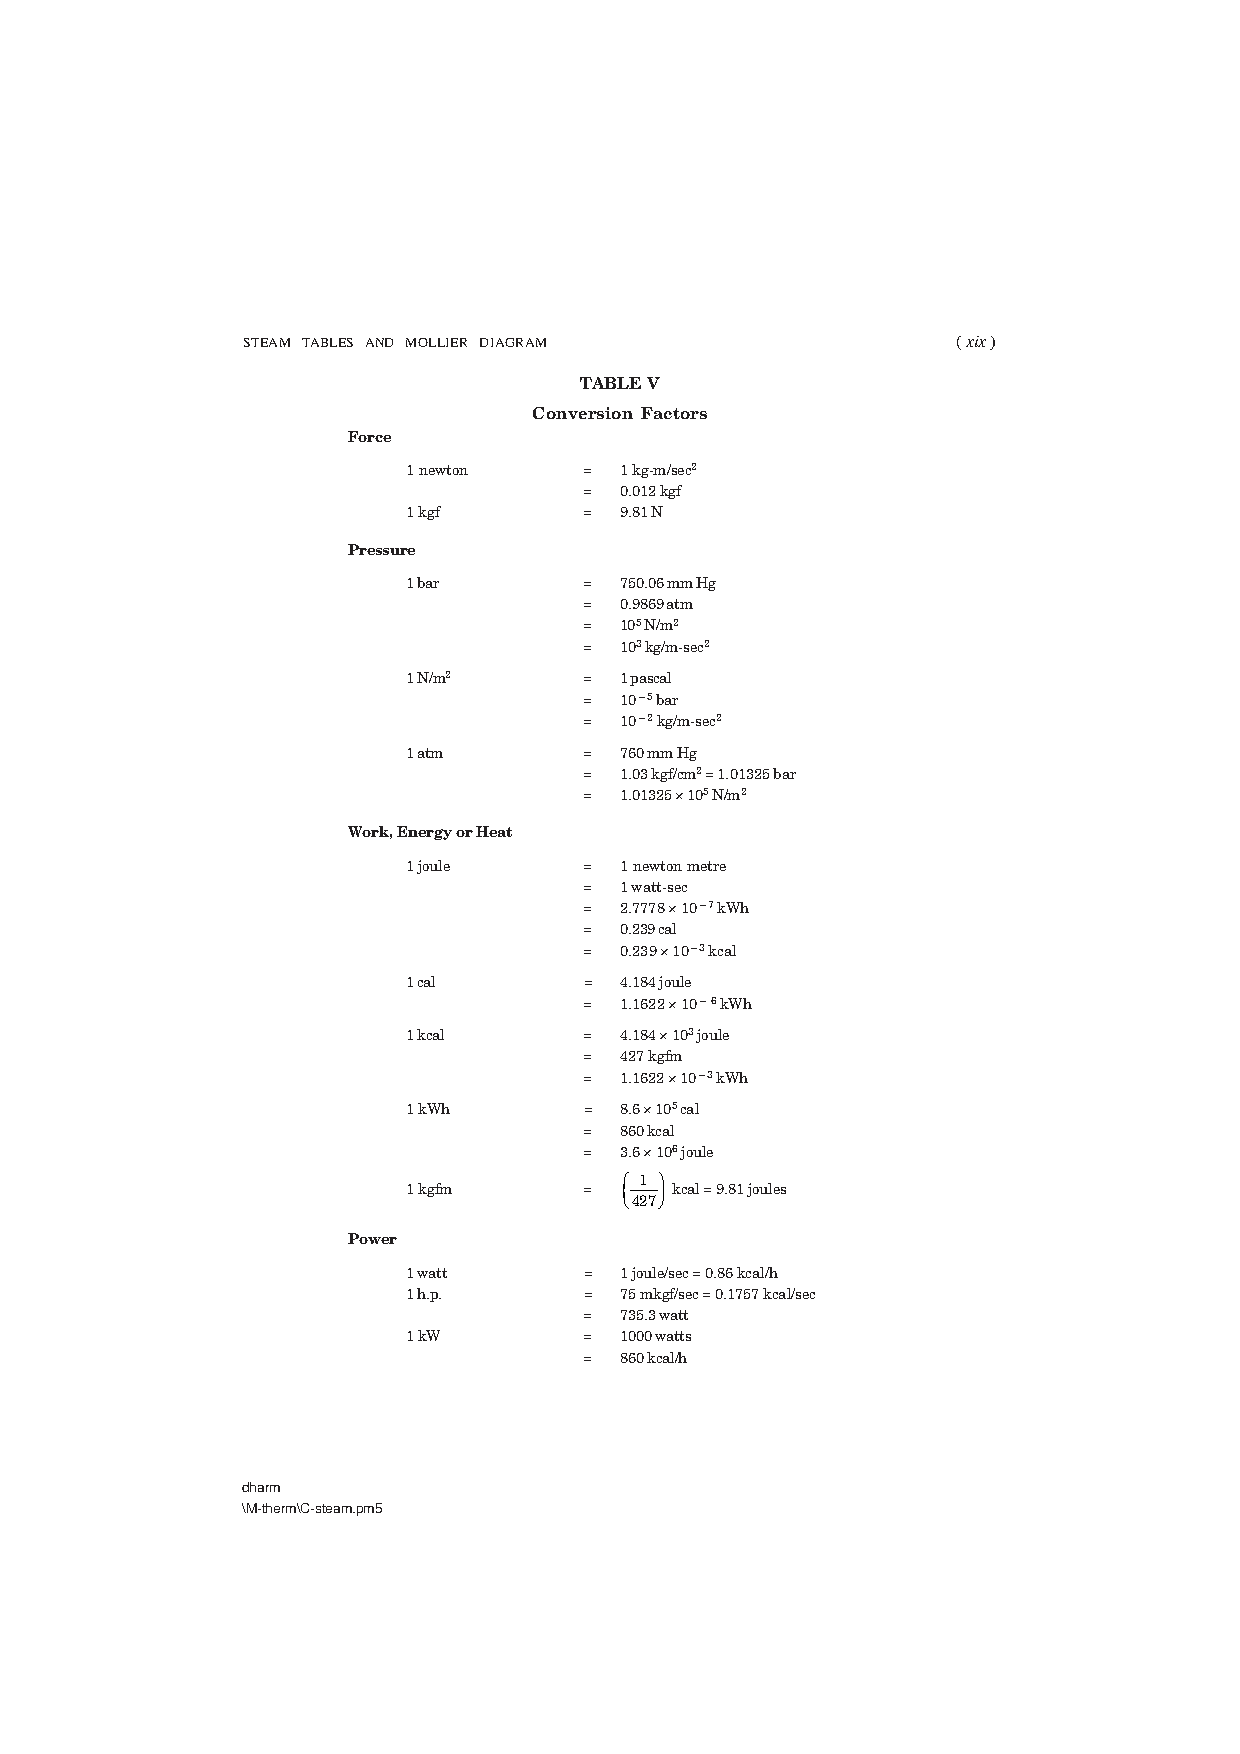
\includepdf[pages=-,fitpaper]{UnitsConversion}
%  \includepdf[pages=-,fitpaper]{SteamTable_2}
%  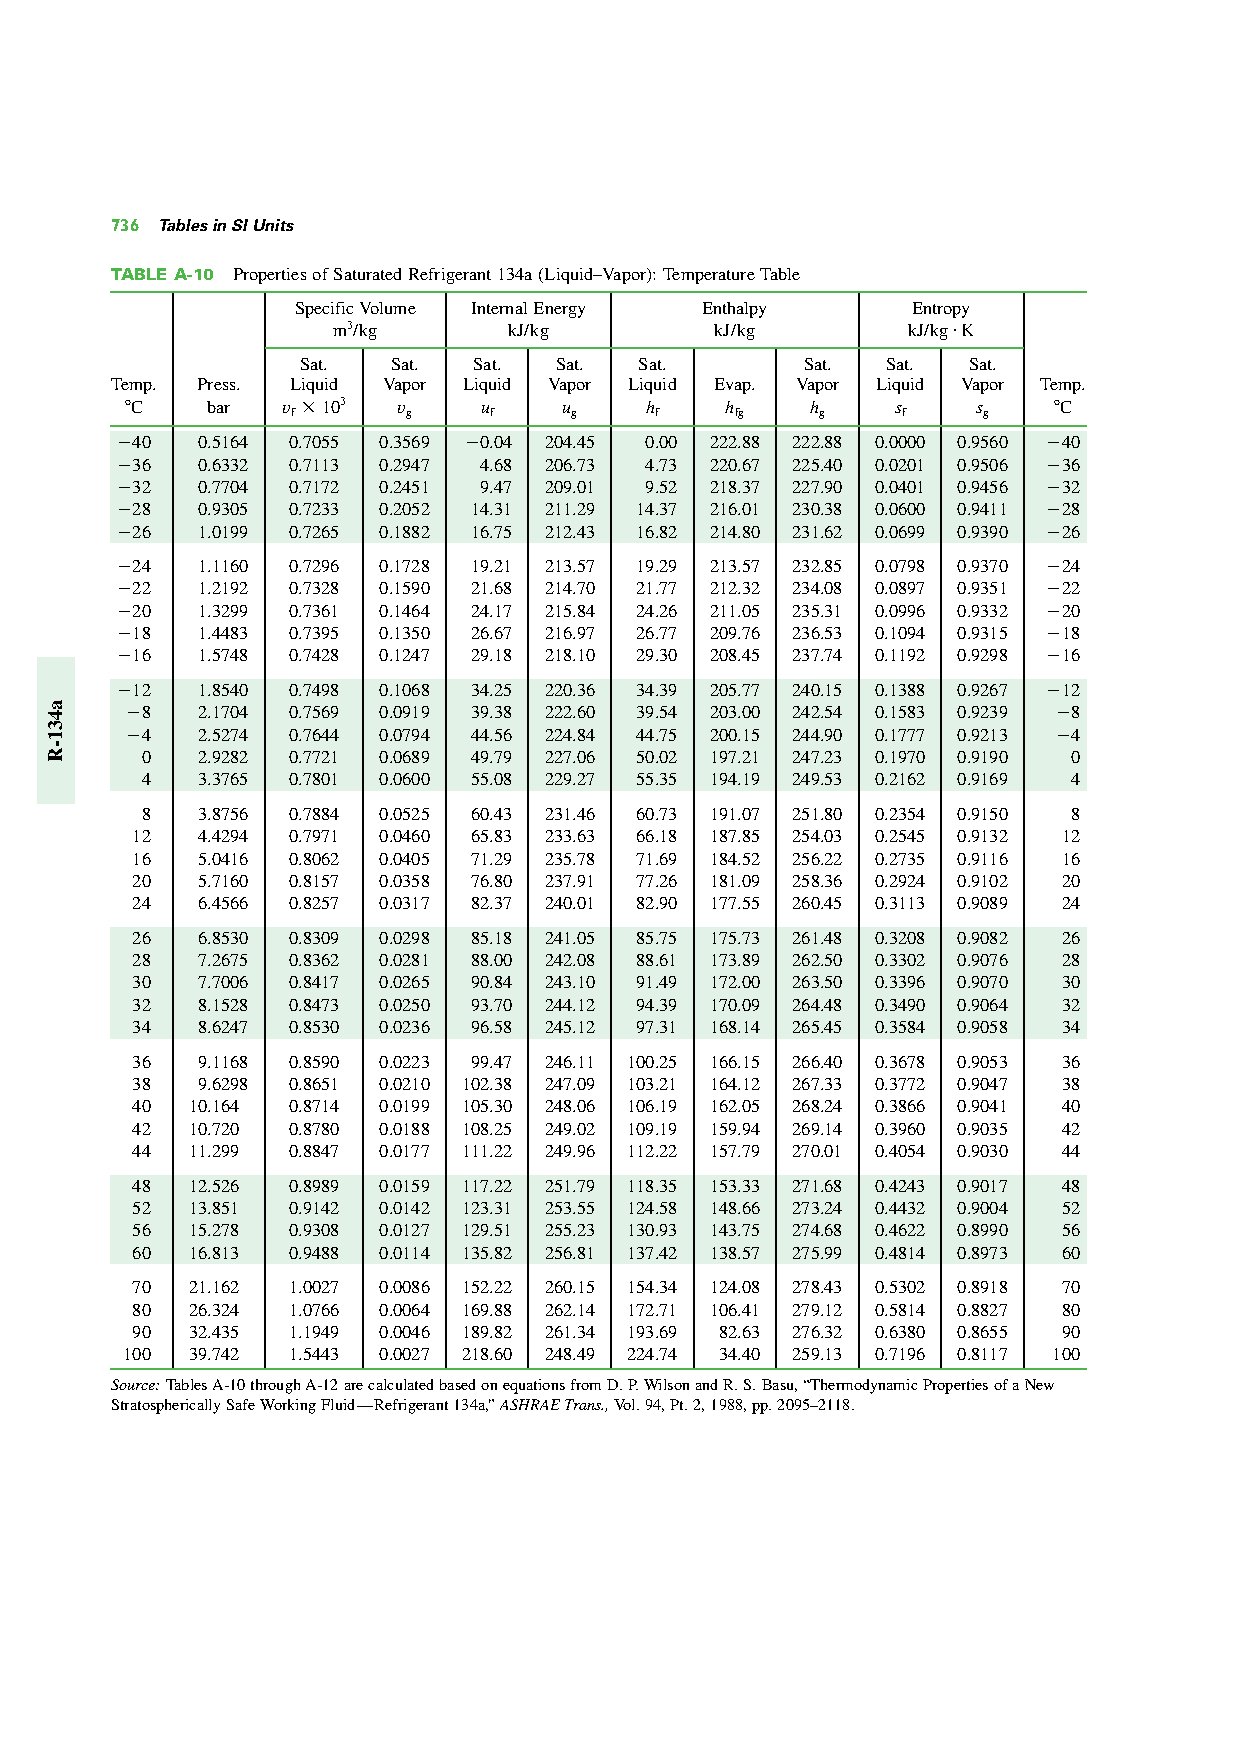
\includepdf[pages=-,fitpaper]{Tables_R134}
%}
%\end{landscape}
%\end{comment}

\end{document}
